\section{Model}
\label{sec:model}

The basic element of our model is a \tg, which represents a graph that
evolves over time.  We define snapshots of an evolving graph in
Section~\ref{sec:model:structure}.  We then formalize the temporal
aspect of our model in Section~\ref{sec:model:time}.  Finally, in
Section~\ref{sec:model:tg} we show how graph evolution is represented
by assigning temporal meaning to sequences of snapshots.

\subsection{Snapshots}
\label{sec:model:structure}

A state of an evolving graph is represented by a snapshot.

\begin{definition}[Snapshot]
A {\em snapshot} $G$ is a pair\\ $(V; E)$, where $V$ is a finite set of
nodes with schema\\ $(\underline{vid}, a_1, \ldots, a_n)$, and $E$ is a
finite set of edges connecting pairs of nodes from $V$, with schema
$(\underline{vid_1}, \underline{vid_2}, b_1, \ldots, b_m)$.
\label{def:sg} 
\vspace{-0.3cm}
\end{definition}

Attributes of vertices and of edges are not restricted to be of atomic
types, but may, e.g., be maps or tuples. However, we require that all
vertices (resp. edges) of $G$ have the same schema, i.e., $V$ and $E$
are homogeneous sets. $G$ may represent a directed or an undirected
graph.  For undirected graphs we choose a canonical representation of
an edge, with $vid_1 \leq vid_2$ (self-loops are allowed).

\begin{definition} [Structural union-compatibility]
Snapshots $G' = (V', E')$ and $G'' = (V'', E'')$ are
union-compatible if $V'$ and $V''$ are union-compatible, and $E'$
and $E''$ are union-compatible.
\label{def:scompat}
\end{definition}

\eat{This is the standard union compatibility definition, which requires
that vertex schema $V$ and edge schema $E$ be the same for $G'$ and
$G''$.}

Several operations of our query language combine two or more snapshots
into a single snapshot. This is done using structural aggregation,
defined next.

\begin{definition} [Structural aggregation]  
A pair of operators $(\gamma^{V}, \gamma^{E}) : {\cal G} \rightarrow
G$ map a collection of snapshots $\cal{G}$ to a snapshot $G$.
$\gamma^{V}$ and $\gamma^{E}$ specify aggregation behavior for the
vertices and for the edges, respectively.  For each, we support two
variants.

\insql{[Any V]} $V(G) = \gamma^{V}_{vid, L}(\bigcup_{G_i \in {\cal G}} V(G_i))$.
Vertices in the resulting snapshot, $G$, are present in {\em any
  snapshot} in ${\cal G}$.

\insql{[All V]} $V(G) = \gamma^{V}_{vid, L}(\bigcap_{G_i \in {\cal G}} V(G_i))$.
Vertices in $G$ are present in {\em all snapshots} in ${\cal G}$.

\insql{[Any E]} $E(G) = \gamma^{E}_{vid_1,vid_2, L}(\bigcup_{G_i \in {\cal G}} E(G_i))$.
  Edges in $G$ are in {\em any snapshot} in ${\cal G}$,
  subject to $vid_1, vid_2 \in V(G)$.

\insql{[All E]} $E(G) = \gamma^{E}_{vid_1,vid_2, L}(\bigcap_{G_i \in
  {\cal G}} E(G_i))$.  Edges in $G$ are in {\em all snapshots} in
${\cal G}$, subject to $vid_1, vid_2 \in V(G)$.

\label{def:sgroup}
\end{definition}

Note that both $\gamma^{V}$ and $\gamma^{E}$ group the respective
collections by their key attributes.  The choice of union
(\insql{Any}) vs. intersection (\insql{All}) for vertices and for
edges is orthogonal, subject to the constraint that an edge is present
in the result only if both vertices it connects are present.  Finally,
note that we did not specify (i) whether ${\cal G}$ is an ordered
collection of snapshots, and (ii) which aggregation operations are
available for non-key attributes of vertices and edges.  We will
address both points in Section~\ref{sec:example}, when we discuss
query language operations that use structural aggregation.

\subsection{Temporal sequences}
\label{sec:model:time}

We next describe how time is represented in our model.  Following the
SQL:2011 standard~\cite{DBLP:journals/sigmod/KulkarniM12}, we adopt
the {\em closed-open} period model, where a period represents all
times starting from and including the start time, continuing to but
excluding the end time.

\begin{definition}[Time period]
A {\em time period} \\$p = [start, end)$ is an interval on the
  timeline, subject to the constraint $start < end$.  We refer to the
  length of time covered by $p$ as its {\em resolution}, which is
  explicitly associated with a {\em unit of time}.
\label{def:period} 
\end{definition}

Examples of time periods are $p_1=[\tpy{2000},\tpy{2001})$ (a 1-year
  period), $p_2=[\tpym{2000}{12},\tpym{2001}{03})$ (a 3-month period)
    and $p_3=[\tpymd{2000}{12}{01},\tpymd{2001}{03}{01})$ (a 90-day
      period).  The unit of time is application-dependent, and will be
      stated explicitly where not clear from context.

Our goal in this work is to support complex analytics over evolving
graphs, under the assumption that all historical data is available in
the database and is read-only.  For this reason we focus on {\em valid
  time}, represented by {\em application-time period} in SQL:2011 ---
the time period during which data is regarded as correctly reflecting
reality.  This is in contrast to {\em transaction time} (or {\em
  system-time period}), which refers to the time period during which a
row is committed to the database.

We now formally define temporal sequences.

\begin{definition} [Temporal Sequence]
A {\em temporal sequence} $P = (p_1, \ldots, p_n)$ is a
sequence of consecutive non-overlapping time periods of the same
resolution, with no gaps.  That is,

\begin{enumerate}
\item $\forall i < n, p_i.end = p_{i+1}.start$, and 
\item $\forall i, j \leq n, p_i.end - p_i.start = p_j.end - p_j.start$.
\end{enumerate}
\label{def:tseq} 
\end{definition}

$P$ may be equivalently described by any two of the following three values:
the start of the earliest period $P.start = p_1.start$, the end of the
latest period $P.end = p_n.end$, and the resolution of any period
$P.res = p_1.end - p_1.start$, specified in appropriate time
units. For convenience, we refer to the number of periods in the
sequence as $P.size$.

For example, $P=([\tpy{1940},\tpy{1945}), \ldots,
  [\tpy{2010},\tpy{2015}))$ represents a temporal sequence with
    $P.start=\tpy{1940}$, $P.end=\tpy{2015}$, $P.res=5$ years, and
    $P.size=15$.

A special sequence $P^{\epsilon}$ is the null sequence, with
$P^{\epsilon}.res=null$, $P^{\epsilon}.start=null$,
$P^{\epsilon}.end=null$, and  $P^{\epsilon}.size=0$.

\eat{\vera{According to the wiki, $[a,a)$ is considered an empty
      set. So if we just follow the standard interval math semantics,
      we can say: A null temporal sequence is a sequence represented
      by the $[p.start,p.end)$ time interval regardless of the
        resolution. By definition it is of size 0.}}

\eat{
\begin{definition} [Temporal Selection]
Operator $\sigma_c P$ returns a temporal sequence $P'$ with $P'.start
\geq P.start$, $P'.end \leg P.end$, and $P',res = P.res$.
\label{def:tsel}
\end{definition}
}

We next define union-compatibility for temporal sequences, and present
two binary operations on temporal sequences.

\begin{definition} [Temporal Union-Compatibility]
Temporal sequences $P'$ and $P''$ are union-compatible if they have
the same resolution, and if we can construct a valid sequence $P$ with
$P.start = min(P'.start, P''.start)$, $P.end = max(P'.end, P''.end)$,
and $P.res = P'.res$.  $P^{\epsilon}$ is union-compatible with any
temporal sequence.
\label{def:tcompat} 
\end{definition}

\begin{example}
\label{ex:ex1}
Consider the following temporal sequences, with year as the unit of
time.

\vspace{-0.3cm}

\begin{eqnarray*}
P_1 & = & ([\tpy{2001},\tpy{2003}),[\tpy{2003},\tpy{2005}))\\
P_2 & = & ([\tpy{2009},\tpy{2010}),[\tpy{2010},\tpy{2011})) \\
P_3 & = & ([\tpy{2008},\tpy{2010}),[\tpy{2010},\tpy{2012}),[\tpy{2012},\tpy{2014}))\\
P_4 & = & ([\tpy{2012},\tpy{2014}),[\tpy{2014},\tpy{2016}))\\
P_5 & = & ([\tpy{2020},\tpy{2022})) \\
\end{eqnarray*}

\vspace{-0.5cm}

$P_1$ and $P_2$ are not union-compatible because the resolution of
  $P_1$ is 2 years, while the resolution of $P_2$ is 1 year.  $P_1$
  and $P_3$ are not union-compatible because, while their resolution
  is the same, it is not possible to construct a valid temporal
  sequence with $P.start=\tpy{2001}$, $P.end=\tpy{2014}$ and a 2-year
  resolution.  Finally, $P_3$, $P_4$ and $P_5$ are pair-wise
  union-compatible.
\end{example}

As our example illustrates, a pair of union-compatible sequences may
not overlap and may not be consecutive.

\begin{definition} [Temporal Intersection] 
Inter-\\section of union-compatible sequences $P'$ and $P''$, denoted $P'
\cap P''$, is a sequence $P$, containing intervals that are in common
to $P'$ and $P''$.  If no intervals are in common to $P'$ and $P''$,
this operation returns $P^{\epsilon}$.
\label{def:tseqand}
\end{definition}
\vspace{-0.1cm}

Continuing with Example~\ref{ex:ex1}, $P_3 \cap P_4 =
([\tpy{2012},\tpy{2014}))$ and $P_3 \cap P_5 = P^{\epsilon}$.

\begin{definition} [Temporal Union]
Temporal union of union-compatible sequences $P'$ and $P''$, denoted
$P' \cup P''$, is the sequence $P$ with $P.start = min(P'.start,
P''.start)$, $P.end = max(P'.end, P''.end)$, and $P.res = P'.res$.
\label{def:tseqor}
\end{definition}
\vspace{-0.1cm}

In Example~\ref{ex:ex1}, $P_3 \cup P_4 =
([\tpy{2008},\tpy{2010}),\ldots,[\tpy{2014},\tpy{2016}))$ and $P_3
    \cup P_5 = ([\tpy{2008},\tpy{2010}), \ldots,
      [\tpy{2020},\tpy{2022}))$.

Finally, we define temporal aggregation, a coarsening operation for sequences.

\begin{definition} [Temporal Aggregation] Operator $\gamma_w(P)$, 
with $w \geq P.res$, returns a temporal sequence $P'$ such that
$P.start = P'.start$, $P.end = P'.end$ and $P'.res = w$, or
$P^{\epsilon}$ if a valid sequence cannot be constructed.
\label{def:tgroup}
\end{definition}

For example, $\gamma_{4y}(P1) = ((2001,2005])$, and
      $\gamma_{3y}(P1)=P^\epsilon$.  Temporal aggregation is semantic,
      e.g., an input sequence that has day as its unit, and 1-day
      resolution, can be coarsened into a sequence with month as its
      time unit, by specifying $w = 1$ month.

\subsection{TGraphs}
\label{sec:model:tg}

\begin{figure*}[th!]
\centering
\begin{minipage}{3.3in}
  \centering
  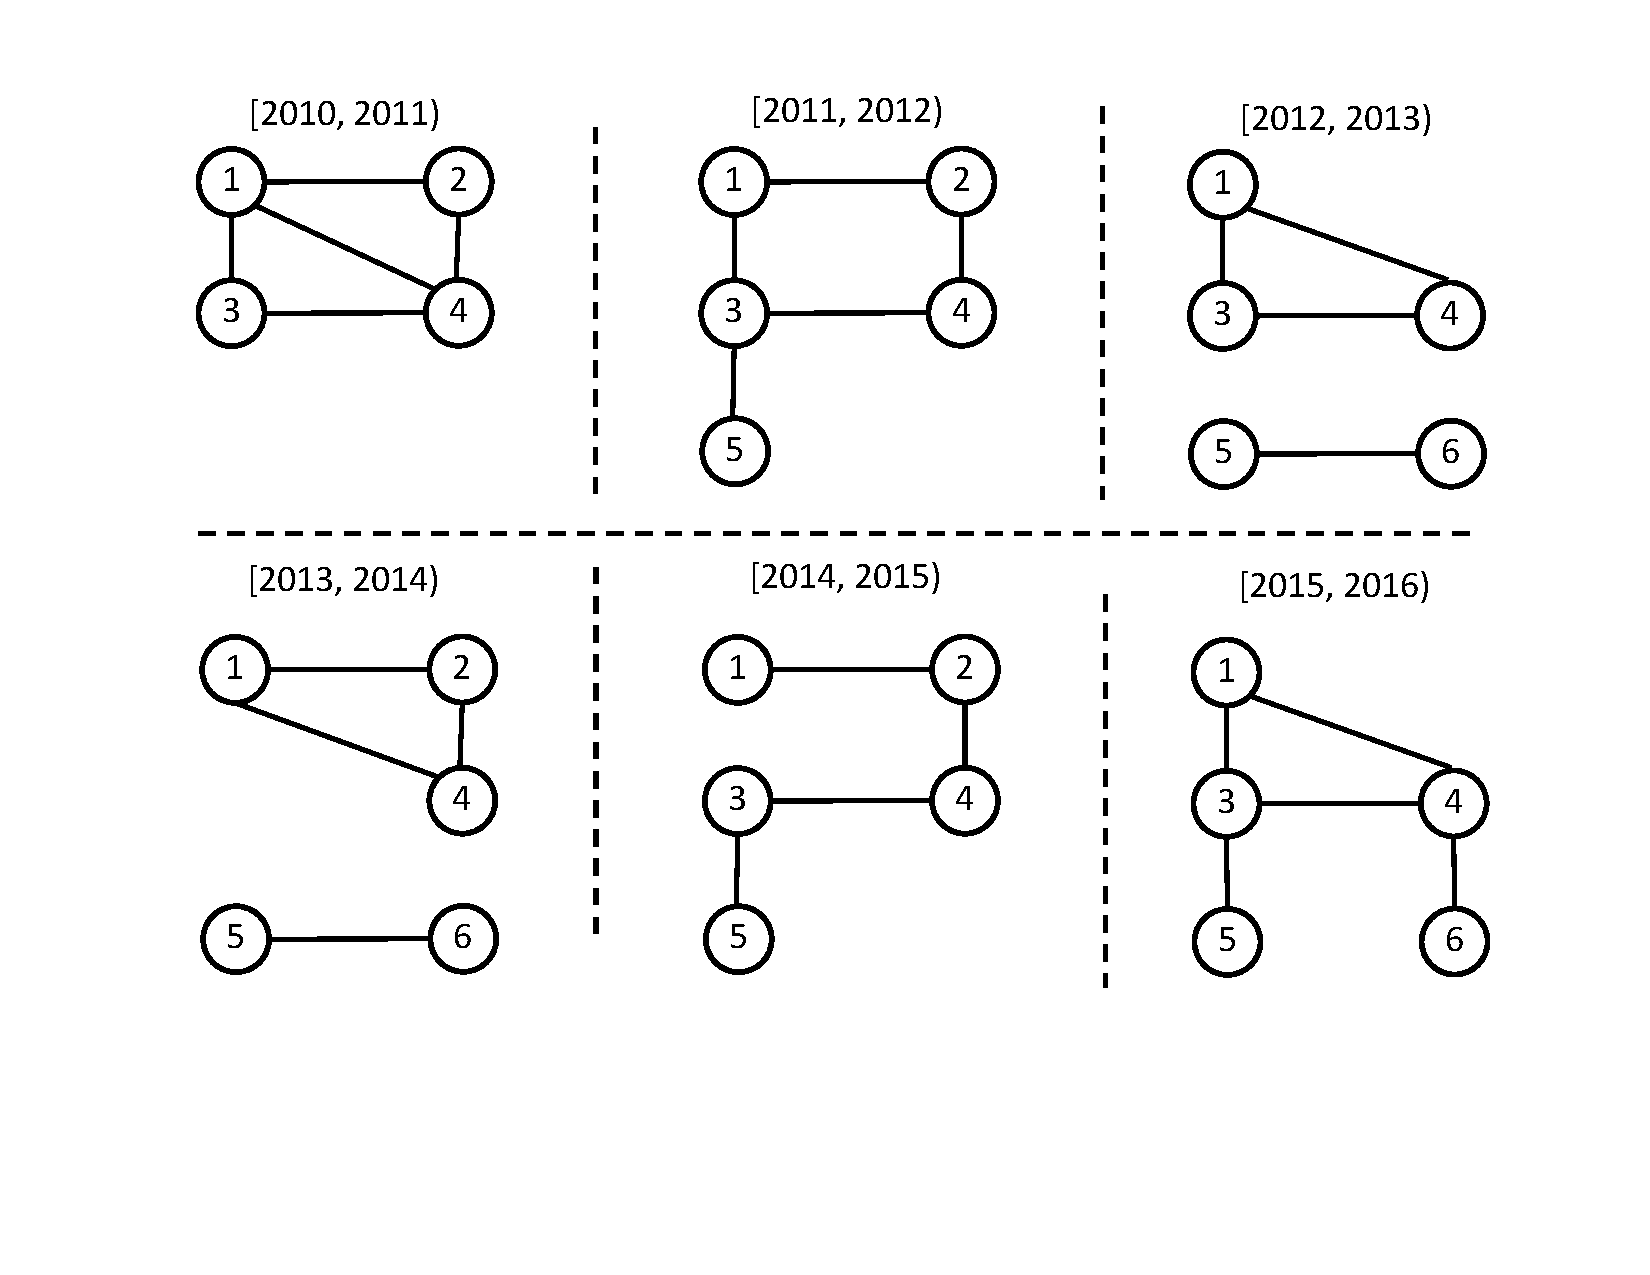
\includegraphics[width=3in]{figs/6snaps.pdf}
  \caption{\tg \insql{T1} with 6 snapshots.}{}
  \label{fig:tg}
\end{minipage}%
\begin{minipage}{3.3in}
  \centering
  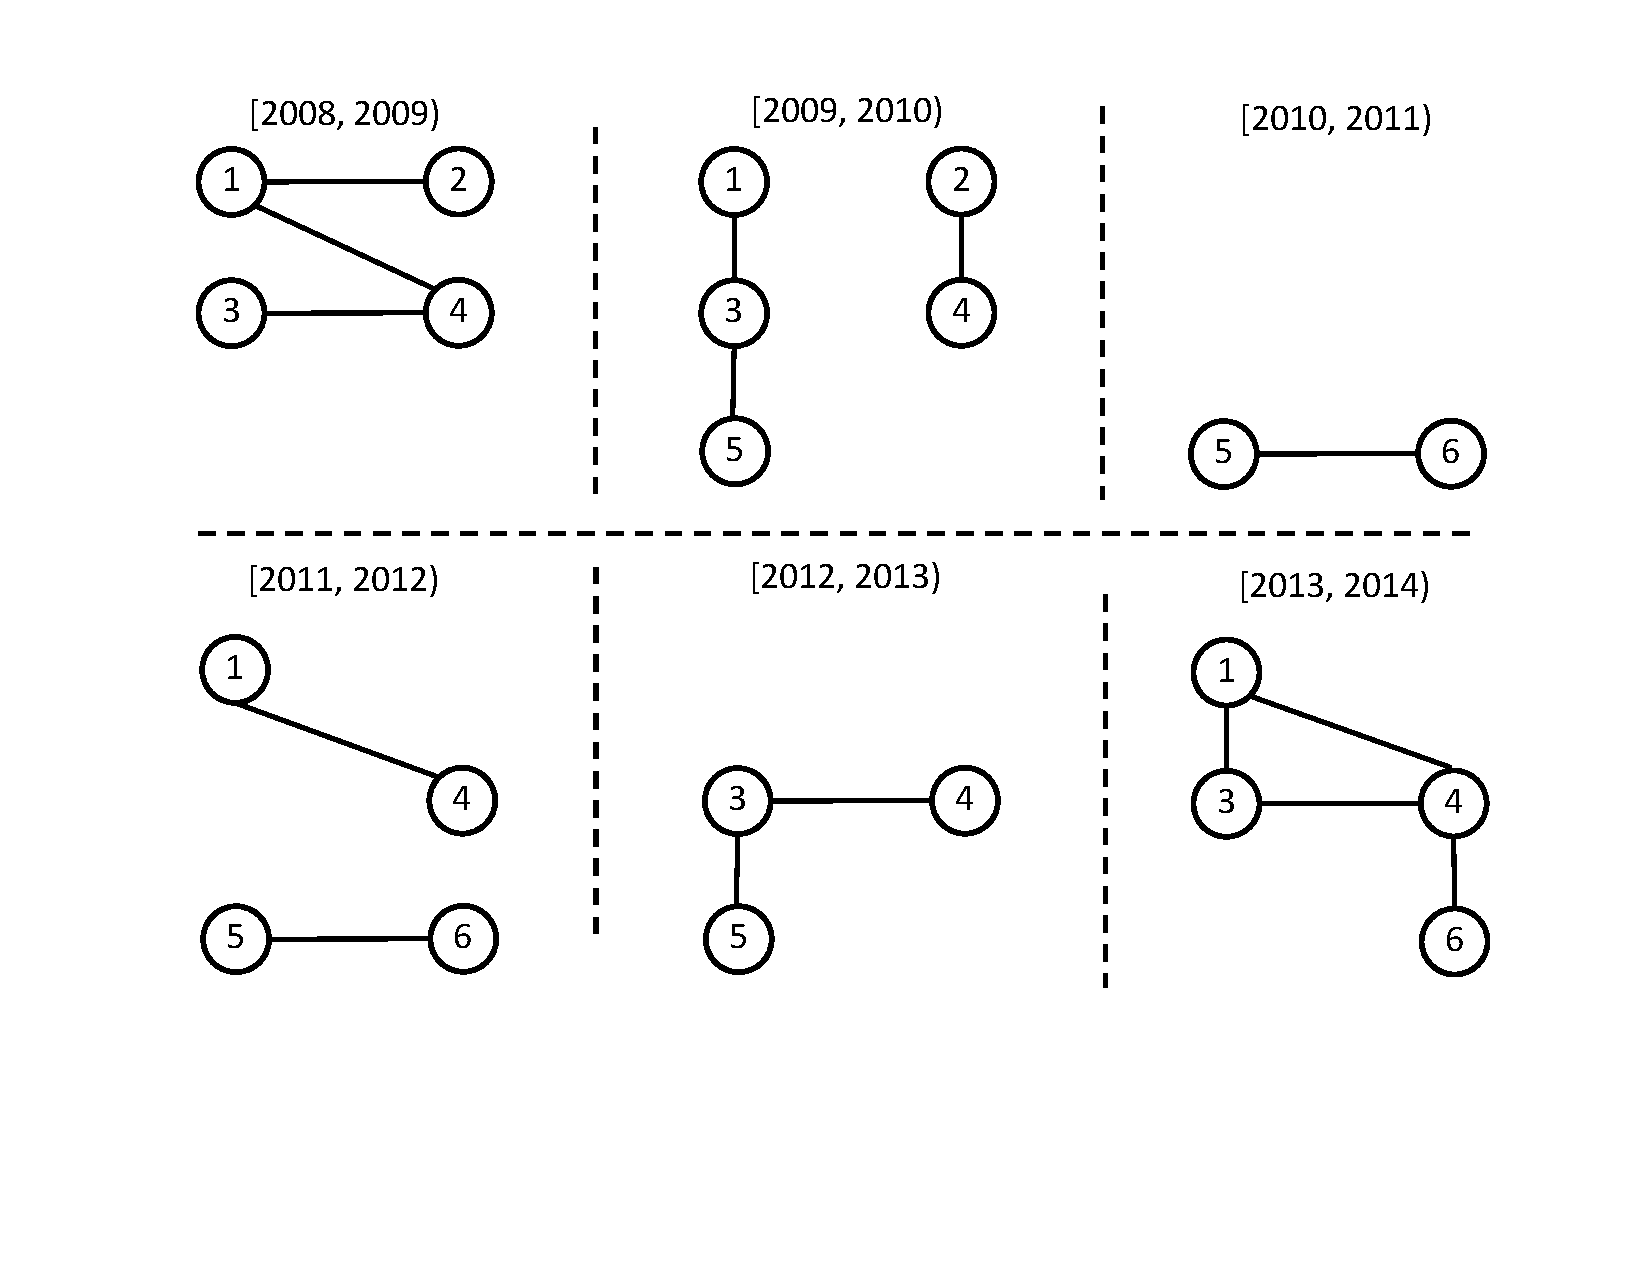
\includegraphics[width=3in]{figs/t2.pdf}
  \caption{\tg \insql{T2} with 6 snapshots.}{}
  \label{fig:tg_t2}
\end{minipage}
\end{figure*}


A snapshot represents a single state of an evolving graph, and is not
time-aware.  Temporal evolution of a graph is represented by a
sequence of snapshots, called a {\em temporal graph}, or \tg for
short.

\begin{definition} [TGraph]
A {\em temporal graph} $T = (G_1, \ldots, G_n; P)$ associates a
sequence of $n$ structurally union-compatible snapshots with a
temporal sequence $P$, such that $P.size = n$.
\label{def:tgraph} 
\end{definition}

Snapshots define the {\em structural schema} of $T$, while $P$
specifies the {\em temporal schema} of $T$.
%
An example of a \tg is given in Figure~\ref{fig:tg}, with instances of
vertex and edge relations for 3 snapshots in Figure~\ref{fig:3ve}.
Importantly, identity of a vertex persists across snapshots in a \tg,
and across \tgs.  For example, vertex with id $3$ represents the same
entity in all snapshots in Figure~\ref{fig:tg} in which it occurs.

To conclude this section, we define union-compatibility for \tgs.

\begin{definition} [\tg Union-Compatibility]
\label{def:tuc} 
$T'$ and $T''$ are union-compatible \tgs if they are both
structurally union-compatible (per Definition~\ref{def:scompat}) and
temporally union-compatible (per Definition~\ref{def:tcompat}).
\end{definition}

The \tg of Definition~\ref{def:tgraph} is the basic element in our
model.  In what follows, we assume that a relation in our database
corresponds to a single \tg, not to a collection of \tgs.  In the next
section we will present the \ql query language that operates on \tgs.




